\حصہ{ایک سے زائد بلا منصوبہ متغیرات کی تقسیمیں}
اگر ایک بلا منصوبہ تجربہ میں ہم ایک مقدار کا مشاہدہ کریں تب ہمیں اس تجربہ کے ساتھ واحد ایک بلا منصوبہ متغیر، مثلاً \عددی{X}، وابستہ کرنا ہو گا۔حصہ \حوالہ{حصہ_شماریات_بلا_منصوبہ_متغیرات} سے ہم جانتے ہیں کہ اس کا مطابقتی تفاعل تقسیم \عددی{F(x)=P(X\le x)} اس تقسیم کو مکمل طور پر تعین کرتا ہے، چونکہ ہر وقفہ \عددی{a<X\le b} کے لئے درج ذیل ہو گا۔
\begin{align*}
P(a<X\le b)=F(b)-F(a)
\end{align*}

اگر ایک بلا منصوبہ تجربہ میں ہم دو مقدار کا مشاہدہ کریں تب ہمیں اس تجربہ کے ساتھ دو بلا منصوبہ متغیرات، مثلاً \عددی{X} اور \عددی{Y}، وابستہ کرنا ہو گا۔مثال کے طور پر فولاد کی راک ویل سختی کو  \عددی{X}  اور اس میں کاربن کی مقدار کو \عددی{Y} ظاہر کر سکتے ہیں۔ہر ایک تجربہ اعداد کی جوڑی \عددی{X=x}، \عددی{Y=y} دے گی جس کو مختصراً \عددی{(x,y)} لکھا اور \عددی{XY} مستوی پر بطور نقطہ دکھایا جا سکتا ہے۔ہم اب ایک مستطیل \عددی{a_1<X\le b_1}، \عددی{a_2<Y\le b_2} پر غور کرتے ہیں (شکل \حوالہ{شکل_شماریات_دو_بعدی_تقسیم})۔اگر ایسے ہر ایک مستطیل کے لئے  ہمیں مطابقتی احتمال
\begin{align*}
P(a_1<X\le b_1,\,\, a_2<Y\le b_2)
\end{align*}
معلوم ہو تب ہم کہتے ہیں کہ \اصطلاح{دو بعدی بلا منصوبہ متغیر}\فرہنگ{بلا منصوبہ!دو بعدی متغیر}\حاشیہب{two-dimensional random variable}\فرہنگ{random!two-dimensional variable} \عددی{(X,Y)} یا بلا منصوبہ متغیرات \عددی{X} اور \عددی{Y} کا \اصطلاح{دو بعدی تفاعل احتمال}\فرہنگ{احتمال!دو بعدی تفاعل}\حاشیہب{two-dimensional probability distribution}\فرہنگ{probability!two-dimensional function} ہمیں معلوم ہے۔تفاعل
\begin{align}\label{مساوات_شماریات_ایک_سے_زائد_الف}
F(x,y)=P(X\le x,Y\le y)
\end{align}
کو اس تقسیم یا \عددی{(X,Y)} کا \اصطلاح{تقسیمی تفاعل}\فرہنگ{تقسیمی!تفاعل}\حاشیہب{distribution function}\فرہنگ{distribution!function} کہتے ہیں۔چونکہ (سوال)
\begin{gather}
\begin{aligned}
P(a_1&<X\le b_1,a_2<Y\le b_2)\\
&=F(b_1,b_2)-F(a_1,b_2)-F(b_1,a_2)+F(a_1,a_2)
\end{aligned}
\end{gather}
لکھا جا سکتا ہے لہٰذا مساوات \حوالہ{مساوات_شماریات_ایک_سے_زائد_الف} تقسیم کو یکتا طور پر تعین کرتا ہے۔
\begin{figure}
\centering
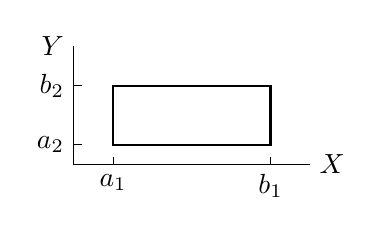
\begin{tikzpicture}
\draw(0,1.5)node[left]{$Y$}--(0,0)--(3,0)node[right]{$X$};
\draw[thick](0.5,0.25) rectangle (2.5,1);
\draw(0.5,0)node[below]{$a_1$}--++(0,0.1);
\draw(2.5,0)node[below]{$b_1$}--++(0,0.1);
\draw(0,0.25)node[left]{$a_2$}--++(0.1,0);
\draw(0,1)node[left]{$b_2$}--++(0.1,0);
\end{tikzpicture}
\caption{دو بعدی تقسیم کا تصور}
\label{شکل_شماریات_دو_بعدی_تقسیم}
\end{figure}

%==================
\جزوحصہء{غیر مسلسل دو بعدی تقسیمیں}
اگر \عددی{(X,Y)} درج ذیل خواص رکھتا ہو تب متغیر \عددی{(X,Y)} اور اس کا مطابقتی تقسیم \اصطلاح{غیر مسلسل}\فرہنگ{غیر مسلسل!تقسیم}\فرہنگ{غیر مسلسل!متغیر}\فرہنگ{discrete!variable}\فرہنگ{discrete!distribution} کہلائے گا۔

\عددی{X,Y} متناہی تعداد یا قابل شمار لامتناہی تعداد کی جوڑی قیمتیں \عددی{(x,y)} اختیار کر سکتا ہے جن کے مطابقتی احتمال مثبت ہوں گے۔ہر ایسا دائرہ کار جس میں ایسی کوئی جوڑی نہ پائی جاتی ہو کا احتمال \عددی{0} ہو گا\حاشیہد{دھیان رہے کہ پہلی خاصیت سے یہ نہیں کہا جا سکتا ہے}۔ 

فرض کریں کہ \عددی{x_i,y_j} ایسی کوئی  جوڑی ہے اور \عددی{P(X=x_i,Y=y_j)=p_{ij}} ہے(جہاں ہم فرض کرتے ہیں کہ \عددی{p_{ij}} کسی مخصوص \عددی{i,j} کی جوڑیوں  کے لئے صفر بھی ہو سکتا ہے)۔ تفاعل
\begin{align}
f(x,y)=
\begin{cases}
p_{ij}& x=x_i,y=y_j\\
0&\text{ورنہ}
\end{cases}
\end{align}
کو \عددی{(X,Y)} کا \اصطلاح{تفاعل احتمال} کہتے ہیں؛ یہاں غیر تابع طور پر \عددی{i=1,2,\cdots} اور \عددی{j=1,2,\cdots} ہیں۔مساوات \حوالہ{مساوات_شماریات_غیر_مسلسل_متغیر_ج} کا مماثل 
\begin{align}
F(x,y)=\sum_{x_i\le x}\sum_{y_j\le y}f(x_i,y_j)
\end{align}
ہے اور مساوات \حوالہ{مساوات_شماریات_غیر_مسلسل_متغیر_پ} کی جگہ درج ذیل شرط ہو گا۔
\begin{align}
\sum_{i}\sum_{j}f(x_i,y_j)=1
\end{align}

مثال کے طور پر اگر ہم ایک روپیہ اور پانچ روپیہ کے سکے اچھال کر 
\begin{align*}
X&=\text{\RL{ایک روپیہ کی خط کی تعداد}}\\
Y&=\text{\RL{پانچ روپیہ کی خط کی تعداد}}
\end{align*}
پر غور کریں تب \عددی{X} اور \عددی{Y} کی قیمت\عددی{0} یا \عددی{1} ہو سکتی ہے اور تفاعل احتمال
\begin{align*}
\text{\RL{ہو گا۔}}\,\, f(x,y)=0\,\,\text{\RL{ورنہ (ان کے علاوہ)}}\,\,f(0,0)=f(1,0)=f(0,1)=f(1,1)=\frac{1}{4}
\end{align*}

%======================
\جزوحصہء{استمراری دو بعدی تقسیمیں}
\عددی{(X,Y)} اور اس کا تقسیم اس صورت استمراری کہلاتے ہیں جب  مطابقتی تفاعل تقسیم کو دوہرا تکمل
\begin{align}
F(x,y)=\int_{-\infty}^{y}\int_{-\infty}^{x}f(x^*,y^*)\dif x^*\dif y^*
\end{align}
کی صورت میں لکھنا ممکن ہو جہاں \عددی{f(x,y)} معین، غیر منفی اور پورے مستوی میں محدود ہے ماسوائے متناہی تعداد کے استمراری قابل تفرق منحنیات پر۔ \عددی{f(x,y)} کو تقسیم کی \اصطلاح{کثافت احتمال} کہتے ہیں۔یوں درج ذیل ہو گا۔
\begin{align}
P(a_1<X\le b_1, a_2<Y\le b_2)=\int_{a_2}^{b_2}\int_{a_1}^{b_1}f(x,y)\dif x\dif y
\end{align}

مثال کے طور پر  (شکل \حوالہ{شکل_شماریات_یکساں_تقسیم_الف})
\begin{align}\label{مساوات_شماریات_یکساں_متعدد_متغیرات_کثافت}
f(x,y)=0\,\text{ورنہ}\,f(x,y)=\frac{1}{k}\,\text{میں ہو تب}\,R\,\text{\RL{مستطیل}} \,(x,y)\,\text{جب}
\end{align}
مستطیل \عددی{R} میں یکساں تقسیم کو ظاہر کرتا ہے؛ یہاں \عددی{k} مستطیل کا رقبہ یعنی \عددی{k=(\beta_1-\alpha_1)(\beta_2-\alpha_2)} ہے۔اس تقسیم کو شکل \حوالہ{شکل_شماریات_یکساں_تقسیم_ب} میں دکھایا گیا ہے۔
\begin{figure}
\centering
\begin{minipage}{0.45\textwidth}
\centering
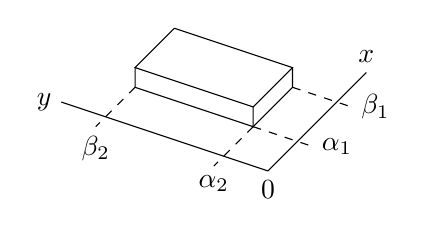
\begin{tikzpicture}[x={(-0.5cm,-0.5cm)},y={(0.75cm,-0.25cm)},z={(0,1cm)}]
\draw(0,0,0.25)--++(1,0,0)--++(0,2,0)--++(-1,0,0)--++(0,-2,0);
\draw(1,0,0.25)--++(0,0,-0.25)--++(0,2,0)--++(0,0,0.25);
\draw(1,2,0)--++(-1,0,0)--++(0,0,0.25);
\draw[dashed] (1,0,0)--++(1,0,0)node[below]{$\beta_2$};
\draw[dashed] (1,2,0)--++(1,0,0)node[below]{$\alpha_2$};
\draw[dashed](0,2,0)--++(0,1,0)node[right]{$\beta_1$};
\draw[dashed](1,2,0)--++(0,1,0)node[right]{$\alpha_1$};
\draw (1.75,2.75)node[below]{$0$}--++(-2.5,0,0)node[above]{$x$};
\draw (1.75,2.75)--++(0,-3.5,0)node[left]{$y$};
\end{tikzpicture}
\caption{یکساں تقسیم (مساوات \حوالہ{مساوات_شماریات_یکساں_متعدد_متغیرات_کثافت}) کا تفاعل احتمال کثافت}
\label{شکل_شماریات_یکساں_تقسیم_الف}
\end{minipage}\hfill
\begin{minipage}{0.45\textwidth}
\centering
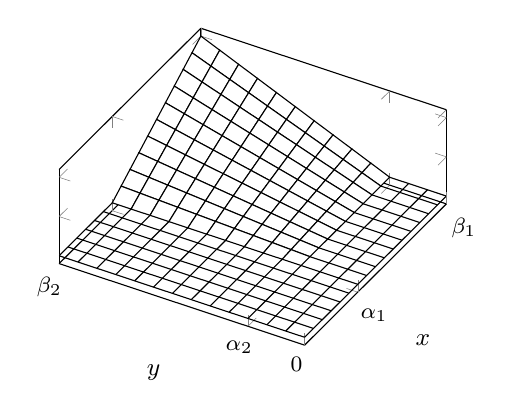
\begin{tikzpicture}
\begin{axis}[small, view={-60}{60},xtick={0.6,1.6},ytick={0,0.6,2.6},xticklabels={$\alpha_1$,$\beta_1$},yticklabels={$0$,$\alpha_2$,$\beta_2$},zticklabels={\empty},xlabel={$x$},ylabel={$y$}]
\addplot3[samples=11,surf,color=white,faceted color=black,domain=0.6:1.6,y domain=0.6:2.6]{(x-0.6)*(y-0.6)};
%the following manually matches the grid lines
\foreach \kk in {0.6,0.8,...,2.6}{
\addplot3 [domain=0:0.6, samples y=1, black,smooth] (x,\kk,0);}
\foreach \kk in {0.6,0.7,...,1.6}{
\addplot3 [domain=0:0.6, samples y=1, black,smooth] (\kk,x,0);}
\foreach \kk in {0,0.2,...,0.58}{
\addplot3 [domain=0:1.6, samples y=1, black,smooth] (x,\kk,0);}
\foreach \kk in {0,0.1,...,0.59}{
\addplot3 [domain=0:2.6, samples y=1, black,smooth] (\kk,x,0);}
\end{axis}
\end{tikzpicture}
\caption{یکساں تقسیم (مساوات \حوالہ{مساوات_شماریات_یکساں_متعدد_متغیرات_کثافت}) کا تفاعل تقسیم}
\label{شکل_شماریات_یکساں_تقسیم_ب}
\end{minipage}%
\end{figure}

%=================
\حصہ{دو بعدی غیر مسلسل تقسیم کے حاشیہ تقسیمیں}
